% Generated by: TimedRegex, Version = 1.0.0.0
% Date 5/14/2024 6:44:16 PM
\usetikzlibrary {automata,positioning}
\scalebox{0.9}{
    % "C(A[5;10]&(BA|A)[1;3])"
    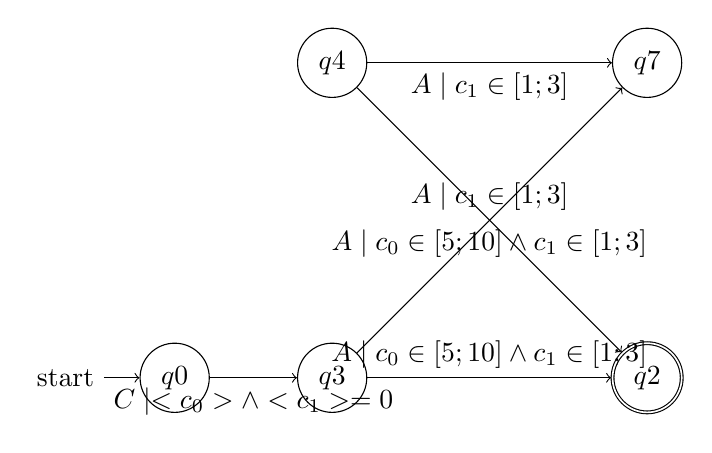
\begin{tikzpicture}[auto]
        \node[state, initial] at (0, 0)(q0){$q0$};
        \node[state] at (2, 0)(q3){$q3$};
        \node[state] at (2, 4)(q4){$q4$};
        \node[state] at (6, 4)(q7){$q7$};
        \node[state, accepting] at (6, 0)(q2){$q2$};
        
        \path[->]
            (q4)edge node[below]{$A\mid c_1\in[1;3]$}(q7)
            (q3)edge node[above]{$A\mid c_1\in[1;3]$}(q7)
            (q4)edge node[below]{$A\mid c_0\in[5;10]\wedge c_1\in[1;3]$}(q2)
            (q3)edge node[above]{$A\mid c_0\in[5;10]\wedge c_1\in[1;3]$}(q2)
            (q0)edge node[below]{$C\mid <c_0>\wedge<c_1>=0$}(q3)
            ;
    \end{tikzpicture}
}

\captionof{figure}{Lightly pruned automaton, to be used as an example.}
\label{fig:prune0}